\subsection{Application of Perching Drones}

\subsubsection{Infrastructure Inspection}

Drones show potential for the automation of inspecting and maintaining infrastructure such as power lines. Chen et al. propose
a method for using lidar mounted on UAVs to measure clearance around transmission line corridors. Performing
checks for encroaching vegetation regularly and quickly is critical for preventing power outages and wildfires caused by encroaching
vegetation. Done manually, this task is slow and inefficient due to the large distances and rough unmanaged terrain that 
must be covered. Drones may perform this task faster as they are unencumbered by the terrain and may move faster
than humans on foot or in land vehicles \cite{chen_automatic_2018}.

Chen et al. developed a clearance measurement system that was deployed on a large UAV; they did not specify the size beyond "large" but the
sensor module they describe building uses a RIEGL VZ-400i LiDAR scanner, which has a specified mass of 9.7kg, and there are other sensors in the
module besides the LiDAR \cite{chen_automatic_2018}. With a mass exceeding 9kg, it is not a device that a typical small quadrotor drone could carry.

There are benefits to using small drones for power line inspection; a small drone could extend its mission time by attaching to the power line
and charging inductively using a design such as the one proposed by Hoang et al. \cite{hoang_autonomous_2024} or Kitchen et al. \cite{kitchen_design_2020}.

The device designed by Hoang et al., shown in Fig. \ref{fig:clasp}, consists of a grasper, a charging circuit and a guidance system. The grasper is passively actuated 
by ribbons that are drawn closed as the drone pushes against the bottom of the power line. Once closer, the grasper is held shut electromagnetically, using
current harvested from the power line. The guidance system implemented uses a radar for measuring distance to power lines and an RGB camera for 
measuring the orientation of the line \cite{hoang_autonomous_2024}.    

\begin{figure}[H]
    \centering
    \begin{subfigure}[b]{\textwidth}
        \begin{subfigure}[b]{0.45\textwidth}
            \centering
            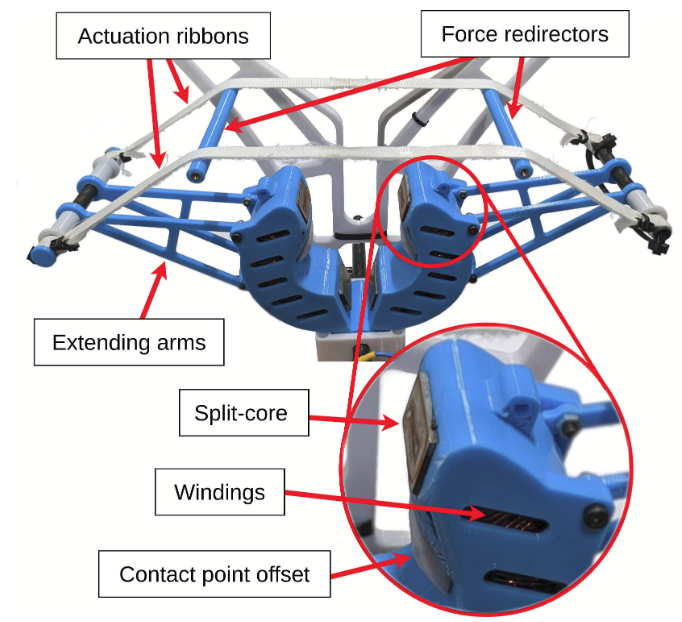
\includegraphics[width=\textwidth]{screenshots/clasp-1.png}
            \caption{Close-up side view of the perching device.}
            \label{fig:clasp:1}
        \end{subfigure}
        \hfill
        \begin{subfigure}[b]{0.45\textwidth}
            \centering
            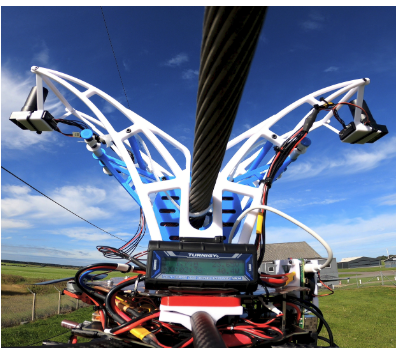
\includegraphics[width=\textwidth]{screenshots/clasp-2.png}
            \caption{Perching device and drone attached to a power line.}
            \label{fig:clasp:2}
        \end{subfigure}
    \end{subfigure}
    \caption{An example of a perching mechanism designed to attach to and charge from power lines. \ref{fig:clasp:1} shows
    a close up of the grasper and charging device, \ref{fig:clasp:2} shows the device and drone attached to a power line.
    Adapted from \cite{hoang_autonomous_2024}.}
    \label{fig:clasp}
\end{figure}

Hoang et al. demonstrated that their design was successful, with a field test lasting over two hours and containing 5 cycles of 
autonomously attaching to a power line, charging, then detaching and resuming flight \cite{hoang_autonomous_2024}.

The device designed by Kitchen et al. is similar to that designed by Hoang et al. The devices design is
illustrated in Fig. \ref{fig:kitchen-grasper}. It consists of a grasper and an inductive charging circuit, 
their grasper is actively actuated rather than passively. Kitchen et al. did not 
develop an autonomous detection and guidance system, and performed their testing in a laboratory environment by 
manually placing a drone on a simulated perch \cite{kitchen_design_2020}.


\begin{figure}[H]
    \centering
    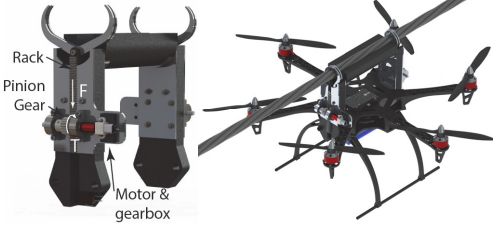
\includegraphics[width=\textwidth]{screenshots/kitchen-grasper.png}
    \caption{An example of an actively actuated perching mechanism designed to attach 
        to and charge from power lines. Adapted from \cite{kitchen_design_2020}.}
    \label{fig:kitchen-grasper}
\end{figure}


\subsubsection{Environmental Monitoring}

Forest canopies contain highly varied microclimates, which support diverse ecosystems and may provide additional resilience to climate change.
These systems are poorly understood, primarily due to the difficulty of observation and data collection. Often canopy cranes are used for
forest observation, however these are costly and not suitable for data collection over a broad area. 
They are also very large, and can themselves cause disruption to the system being studied \cite{nakamura_forests_2017}.
Other methods for tree canopy access include constructing towers, scaffolds, or aerial walkways through the tree canopy, 
though these methods are also inflexible, and they do not permit access to all levels of the canopy. Climbing can also 
allow researchers access to the canopy, but this requires training, poses a safety hazard, and only permits
access to lower levels where branches will support a humans weight \cite{parker_access_1992}.

Tropical forests are a primary target for global restoration and carbon sequestration efforts,
so increasing knowledge of these forests is critical for understanding how to protect them and the global climate \cite{mrema_ten_2020}.
Drones have potential as methods of collecting better data about forests. Being mobile, they can collect data over larger areas without the
need to construct replicated observation stations. The density of obstacles in a forest canopy can be a challenge for drones, but methods
to navigate similar environments have been proven \cite{mulgaonkar_robust_2018,tan_design_2017,liu_mini-drone_2023}. Two major problems
remain for using drones in ecological data collection: they are very loud and disruptive to wildlife being studied
\cite{jenni-eiermann_unmanned_2017,bennitt_terrestrial_2019}, and they have a short flight time due to their high power consumption.

Drones with perching features could allow sensors to be deployed in tree canopies without being limited by short flight time
or disturbing wildlife with loud noise. Kirchgeorg et al. designed a passive perching mechanism for this purpose, 
to attach a drone to tree branches using high-friction spines. Their design was intended to be resilient to
misalignment and avoid needing large open spaces for maneuvering and positioning \cite{kirchgeorg_hedgehog_2022}.
A number of other perching mechanisms targeting tree branch perching have been developed, such as the overhead grasping 
device designed bey Kirchgeorg et al. \cite{kirchgeorg_soft_2023} or the grapple device designed by Nguyen et al. \cite{nguyen_passively_2019}.

The possible uses for drone perching in ecological data collection may be overstated. A Michigan state affiliated researcher 
with experience in using drones for data collection shared that the main benefit of drones in their field is not the ability
to position sensors for long term collection, but their ability to sample a large area in a short amount of time. Additionally,
a drone and sensor payload often represents a large portion of an environmental researchers budget, and they are not likely
to be comfortable leaving it unattended in a tree \cite{_toto_cite_interview_}. Though it is worth considering that the 
forests of Michigan may provide a very different set of challenges for data collection than a tropical rainforest, and 
perching drones may still have use in specific environments.

Where perching an entire drone may be undesirable, a device such as that designed by Geckeler et al. could be used
to attach only a small and low-cost sensor payload, with the drone acting only as a delivery and retrieval mechanism.
Their design is passively actuated, using an elastic coil to wrap around a perch once the device is pressed against the
perch by a drone \cite{geckeler_bistable_2022}. 


\subsubsection{Networking}

Another application of drone perching is to establish temporary sensor networks using drone swarms. Seiber et al. propose using
swarms of drones equipped with air quality sensors to monitor the perimeter of hazardous gas plumes, such as might be 
released from a toxic material spill. This provides two benefits compared to manual data collection: removing humans
from identification of the plume boundaries reduces risk that humans will be exposed to toxins, and a network connected
drone swarm can provide lower latency than manual data collection \cite{seiber_tracking_2018}.

Seiber et al. propose a drone design that is constantly in flight, providing a visual cue to the perimeter of a plume
that first responders can use; since the drones are programmed to fly towards the outer edge of the gas cloud,
first responders simply look up to see where the drones currently are \cite{seiber_tracking_2018}. Liu et al. point out
that the short battery life of most drones is a limiting factor to this approach, and propose using perching drones for 
establishing sensor and communication networks. Using drones with perching abilities provides the benefit of quickly deploying
a network in hazardous or hard to reach areas, while extending mission time by shutting down flight systems once a perching 
location has been found \cite{liu_perching_2022}.


\subsection{Modes of Perching}

Meng et al. identify 3 primary modes of drone perching in their review \cite{meng_aerial_2022}. The modes identified are:
\begin{itemize}
    \item Grasping based perching mechanisms.
    \item Embedding based perching mechanisms.
    \item Attaching based perching mechanism.
\end{itemize}

\subsubsection{Grasping}

Grasping based mechanisms use attachments that can grip a perch with enough force to hold a drone stationary.
Often they are inspired by birds claws and are designed to allow a drone to sit on top of its perch. One benefit
of such a method is that the grasper can, if correctly designed, serve dual use as a perching device as well as
a grasper for carrying or manipulating objects \cite{meng_aerial_2022}.

One example of a grasping based mechanism is proposed by Chi et al., and shown in Fig. \ref{fig:claw}. It aims 
to imitate the biomechanics of bird legs. The design proves capable of holding a 2kg mass stationary on a perch, 
both in static testing and when dropped onto a perch \cite{chi_optimized_2014}.

\begin{figure}[H]
    \centering
    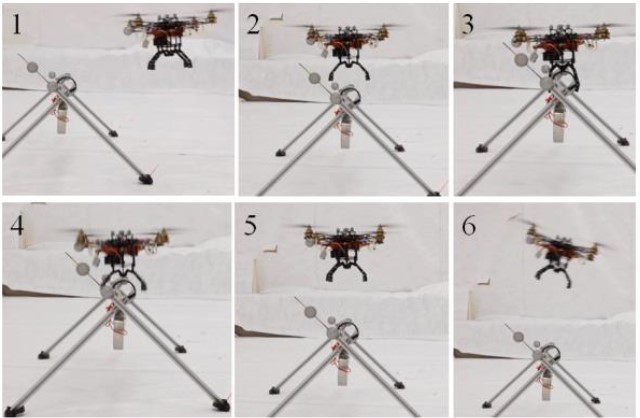
\includegraphics[width=\textwidth]{screenshots/claw.jpg}
    \caption{An example of a claw-like perching mechanism, where the drone lands on a perch and remains fixed by closing the claw. Adapted from \cite{chi_optimized_2014}.}
    \label{fig:claw}
\end{figure}

Though many grasping based perching mechanisms are inspired by avian biomechanics, some take a different approach and attach a drone to a perch from the bottom via a mechanical clasping mechanism.
The device proposed by Hoang et al. shown in Fig. \ref{fig:clasp}, which is intended for use in power line inspection, is such a device.
It uses ribbons to passively close an electromagnetic clasp once the drone has approached the appropriate position below a power line. 
Once closed, current harvested from the power line can be used to keep clasp closed as well as recharge the drone \cite{hoang_autonomous_2024}.

The device designed by Kominami et al., shown in Fig. \ref{fig:passive}, is another grasping type device that grasps a perch beneath the drone. 
A distinguishing feature of this design is that it is passively driven; the grasping force is provided by the weight of the drone on top of the grasper \cite{kominami_detection_2023}.

\begin{figure}[H]
    \centering
    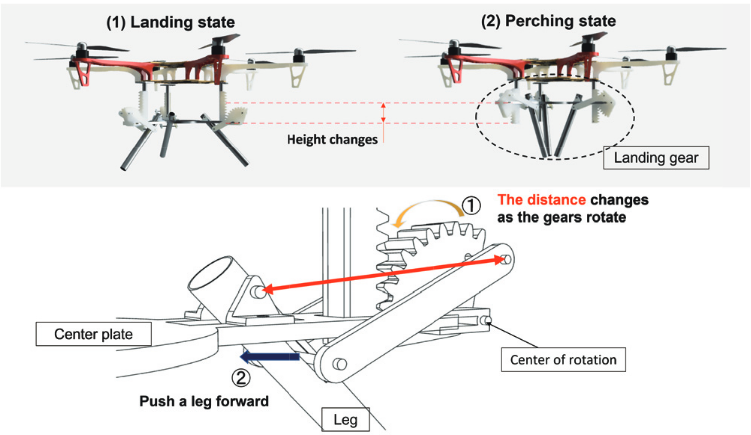
\includegraphics[width=\textwidth]{screenshots/passive.png}
    \caption{A passively actuated perching mechanism that uses the drones weight to provide the grasping force. Adapted from \cite{kominami_detection_2023}.}
    \label{fig:passive}
\end{figure}


\subsubsection{Embedding}

Embedding based perching mechanisms take advantage of the texture of a surface and spikes on the drone to attach the drone to the surface. 
This works similarly to how many insects climb surfaces, by using tiny spikes that grasp onto microscopic cracks or bumps on a surface. 
This method can allow drones to perch on vertical surfaces, though it is not universal to all surface types and 
can provide less stability than grasping based methods \cite{meng_aerial_2022}. 

Distinguishing between grasping and embedding mechanisms can be simply a matter of scale, as embedding mechanisms often operate like very small graspers.
Fig. \ref{fig:gripper} illustrates a device proposed by Roderick et al. which is designed to grip the bark of a tree \cite{roderick_bioinspired_2017}.
While it does not attach by grasping an actuator around the circumference of a tree like a typical grasping based device would, Fig. \ref{fig:gripper}
shows that it is still operating by grasping onto smaller scale features.

\begin{figure}[H]
    \centering
    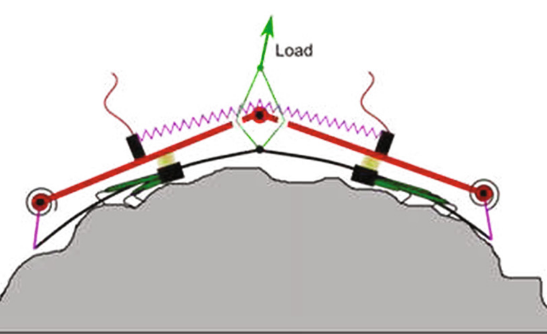
\includegraphics[width=\textwidth]{screenshots/bark gripper.png}
    \caption{Perching device designed to attach to the vertical side of a tree trunk. Adapted from \cite{roderick_bioinspired_2017}.}
    \label{fig:gripper}
\end{figure}


\subsubsection{Attaching}

Attaching based perching devices use adhesives, electromagnetics, electrostatics, or vacuum cups to attach a drone to a surface. Such methods
can work with both smooth and rough surfaces, unlike grasping or embedding methods, and can attach drones above, below, or to the side of a perch
object \cite{meng_aerial_2022}.

One example of such a device is shown in Fig. \ref{fig:electroadhesive}, designed by Gaule et al. It uses electrostatic adhesion to 
attach an insect inspired micro UAV to the underside of an object \cite{graule_perching_2016}.

\begin{figure}[H]
    \centering
    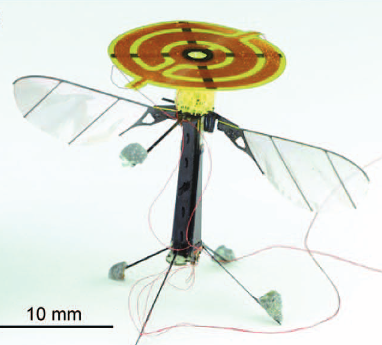
\includegraphics[width=\textwidth]{screenshots/electroadhesive.png}
    \caption{Example of an attaching based perching device that uses electrostatic adhesion. Adapted from \cite{graule_perching_2016}.}
    \label{fig:electroadhesive}
\end{figure}


\subsection{Perch Detection Methods}

Kominami et al. designed a perch detection method in conjunction with their passive grasping device shown in Fig. \ref{fig:passive}.
Their detection method is designed to detect long thin features that the grasper is designed to land on, such as signs and fences. 
Using a RealSense D405 RGB-D camera they implement the following image processing pipeline:

\begin{enumerate}
    \item RGB data is processed with a Hough transform to identify the top and bottom edge of a long thin board.
    \item The depth data is used to measure a depth profile of the board along a line perpendicular to the two edges.
    \item The shape of the depth profile is used to confirm the type of object detected.
    \item If a suitable object is confirmed, then the location of its top is returned.
\end{enumerate}

This method proved capable of identifying the board to perch on, though it suffers from being unable to identify a thin board when the drone is directly
above it \cite{kominami_detection_2023}.


An alternative detection method proposed by von Frankenberg and Nokleby uses a RANSAC method to detect cylindrical perches in a point cloud. They used a Microsoft
Kinect to acquire 3D point clouds and processed them using the following sequence:
\begin{enumerate}
    \item Downsample and crop point cloud.
    \item Identify possible lines with a RANSAC approach.
    \item Remove any lines that make an angle with the x-y plane steeper than $30^\circ$.
    \item Scan the length of each detected line and remove lines that have gaps where no points are detected.
    \item Scan the length of each detected line and remove lines that have points too close to the line, which indicates obstructions.
\end{enumerate}

The authors note that their algorithm was successfull in detecting a suitable test target, however it suffered from high computation time.
Using an Intel i7-4770 3.40 GHz 4 core processor their method was able to collect measurements at 10Hz with point clouds containing up to 5000
points, however processing time quickly increases as the number of point grows or if the point cloud becomes dominated by planar objects (their test 
scene shows only 2 ladders and a pair of pipes, all of which produce only thin line-like shapes in the point cloud). Additionally, the randomness
of the RANSAC method they use leads to the target object not being detected in every frame because its points were not selected in every frame \cite{von_frankenberg_detection_2020}.